\chapter{Selection and Cutting in the Multigrid} \label{chapter:multigrid_selection_and_cutting}
In this chapter the details of the selection and cutting procedure will be explained. Moreover, we will show how to keep track of the inverse mapping while adding fundamental and special grid regions to the multigrid. For the sake of clarity, we will ignore the special grid regions in most parts of this chapter and come back to them in the last part of this chapter.
\section{Cutting procedure}\label{sec:cutting_procedure}
\index{Cutting procedure}
As it was shown in the last chapter, each grid region has a center point $\omega_c$, a buffer region boundary below and above the center point $d\omega_-$ and $d\omega_+$, and a upper an lower boundary $\omega_l$ and $\omega_r$. If there is overlap between two grid regions, the boundaries and grid parameters have to be adapted such, that the resolution remains constant across the cutting point. We consider two overlapping grid regions and indicate the grid region with the smaller center point by a superscript $l$ for left, and the other one by a superscript $r$ for right (see figure \ref{fig:cutting_gr}).

\begin{figure}[h]
	\centering
	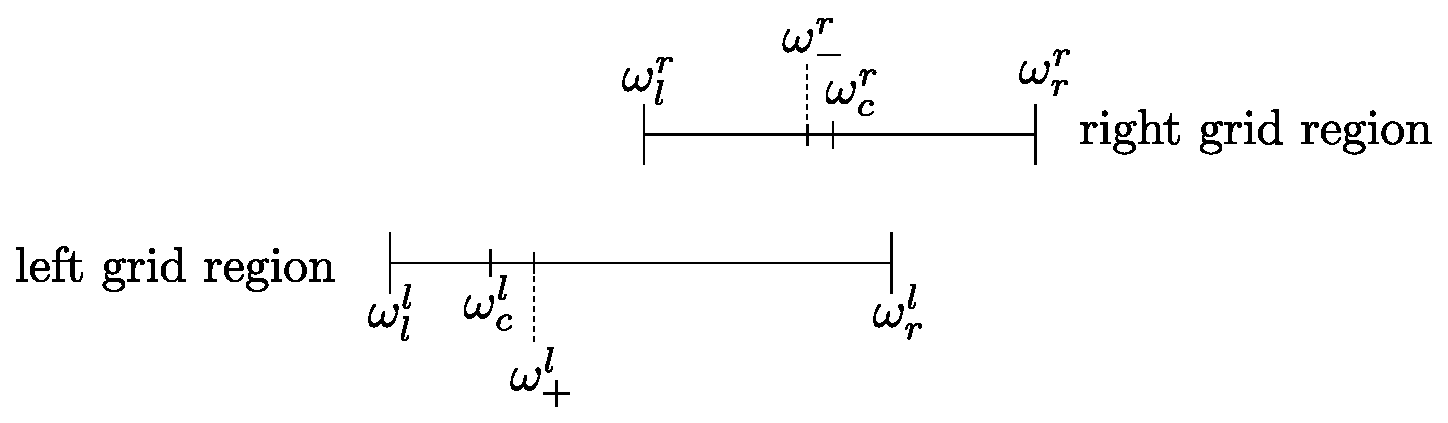
\includegraphics[width=0.8\textwidth]{pics/cutting_gr.eps}
	\caption{Nomenclature for the cutting of two intersecting grid regions}
	\label{fig:cutting_gr}
\end{figure}

The cutting point must be right from the center point of the left grid region plus a small grid dependent buffer, this point is $\omega_+^l$. It also has to be left from the center point of the right grid region minus a small grid dependent buffer, this point is $\omega_-^r$. Moreover the cutting point must not exceed the right boundary of the left grid region $\omega_r^l$ while at the same time it must not fall below the left boundary of the right grid region $\omega_l^r$. Therefore the cutting point $\omega_s$ must lie inside the interval
\begin{equation}\label{eqn:cutting_point_boundaries}
	\omega_s \in [\,max(\omega_+^l, \omega_l^r)\,,\;\; min(\omega_-^r, \omega_r^l)\,]\;:=I
\end{equation}
In this interval, the grid point density of the left grid region $\frac{di}{d\omega}|_l$ is monotonically decreasing and the grid point density of the right grid region $\frac{di}{d\omega}|_r$ is a monotonically increasing. The cutting point should be that point, where the grid point densities of both grid regions become equal
\begin{equation}\label{eqn:cutting_point}
	\left. \frac{di}{d\omega}\right|_l(\omega_s) \stackrel{!}{=} \left. \frac{di}{d\omega}\right|_r(\omega_s)
\end{equation}
This equation, can be solved analytically for all combinations of equidistant, tangential and logarithmic grid regions. This is done in appendix \ref{sec:app_cutting_points}. The calculated cutting point does not always lie inside the interval $I$. In such a case one has to put more thought in what to do. This is done in the following where we list all possibilities which can occur if a solution to equation \ref{eqn:cutting_point} exists (see also figure \ref{fig:cutting_gr_cases}):

\begin{itemize} % itemize because cases label should be in agreement with source code
	\item{\bf Case A}: $\omega_s \in I$: If the calculated cutting point lies inside the interval $I$, both grids are cut at this particular point.

	\item{\bf Case B}: $\omega_s \notin I$ and $\omega_s \in [\omega_l^r, \omega_+^l)$ and $\omega_s \notin (\omega_-^r, \omega_r^l]$: This means, that the maximal resolution of the left grid is smaller than the resolution of the right grid at $\omega_+^l$. Therefore the purpose of the left grid region is assumed to be fulfilled by the right grid region, and the left grid region is skipped.

	\item{\bf Case C}: $\omega_s \notin I$ and $\omega_s \notin [\omega_l^r, \omega_+^l)$ and $\omega_s \in (\omega_-^r, \omega_r^l]$: This means, that the maximal resolution of the right grid is smaller than the resolution of the left grid at $\omega_-^r$. Therefore the purpose of the right grid region is assumed to be fulfilled by the left grid region, and the right grid region is skipped.

	\item{\bf Case D}: $\omega_s \notin I$ and $\omega_s \in [\omega_l^r, \omega_+^l)$ and $\omega_s \in (\omega_-^r, \omega_r^l]$: The distance between both center points is so small, that the calculated cutting point lies inside both buffer regions. Here, the grid region with the smaller maximal resolution is skipped.

	\item{\bf Case E}:  $\omega_s \notin I$ and $\omega_s < \omega_l^r$. The resolution of the right grid region is greater than the resolution of the left grid region over the whole range of the right grid region, even at $\omega_l^r$. Therefore the right grid region will not be cut at all. If there is still enough space for the left grid region, i.e. if $\omega_+^l\leq\omega_l^r$, the left grid region will be cut at $\omega_l^r$. If not, the left grid region will be skipped.

	\item{\bf Case F}:  $\omega_s \notin I$ and $\omega_s > \omega_r^l$. The resolution of the left grid region is greater than the resolution of the right grid region over the whole range of the left grid region, even at $\omega_r^l$. Therefore the left grid region will not be cut at all. If there is still enough space for the right grid region, i.e. if $\omega_-^r \geq \omega_r^l$, the right grid region will be cut at $\omega_r^l$. If not, the right grid region will be skipped.
\end{itemize}

\begin{figure}[h]
	\centering
	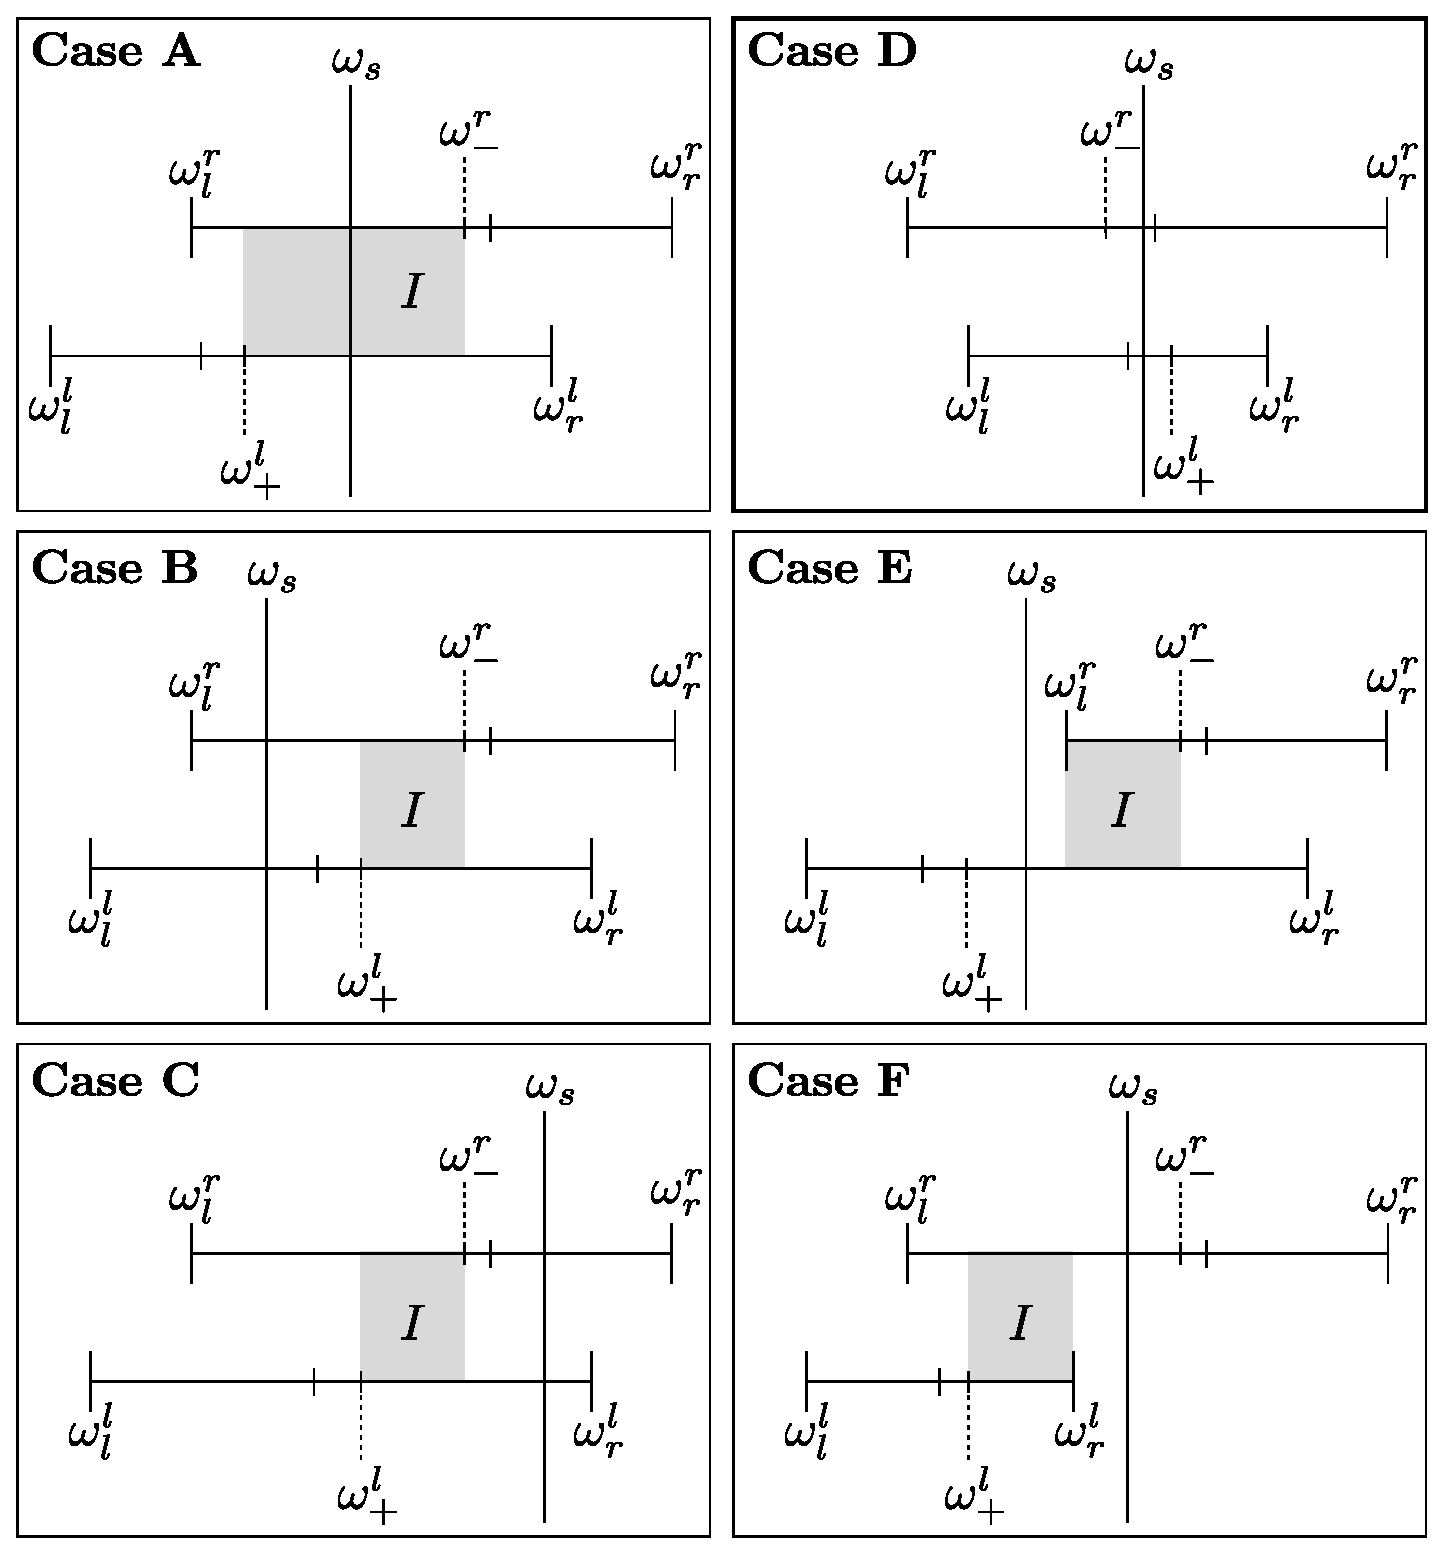
\includegraphics[width=0.8\textwidth]{pics/cutting_gr_cases.eps}
	\caption{Different cases for the cutting of two overlapping grid regions}
	\label{fig:cutting_gr_cases}
\end{figure}

Of course there are cases, in which a solution to equation \ref{eqn:cutting_point} does not exist. If this happens, the lowest resolution of one grid region is higher than the highest resolution of the other. This is basically the same situation as in the cases E and F in the above listing. The only difference is, that one has to find out which of the both grid regions should be favored. This is done by comparing the maximal resolution of both grid regions. Afterwards, one checks if there is still enough space for the non-favored grid region. If this is the case, it will be cut, otherwise it will be skipped  (see cases E and F).

By cutting a grid region at a given cutting point, one has to adjust the grid parameter of this grid region such, that the maximal resolution remains the same. This adaption is different for the equidistant, tangential and logarithmic grid regions and is explained in appendix \ref{sec:app_cutting_gr}.

Grid regions which have overlap with the boundaries of the basic grid region are selected and cut in a similar way. If the center point is outside of these boundaries, the grid region is skipped. It is also skipped if there is not enough space between the buffer region and the boundaries (like in the cases E and F). Otherwise it is cut at the boundaries.

So far, we have only considered two overlapping grid regions. We have shown how the selection an cutting procedure works in this case. Treating multiple overlapping grid regions is a bit more complicated, but can be boiled down to the two grid region case in the end. We will show how this is done in the following. At first, all grid regions are sorted with respect to their center points. Afterwards one iterates through all neighboring pairs of grid regions, starting from the left, i.e. the grid region with the lowest center point, and applies the selection and cutting procedure to each of this pairs. If none of both grid regions is decided to be skipped, the algorithm proceeds to the next pair of neighboring grid regions. Otherwise, if one of the grid regions has to be skipped, it is necessary to re-evaluate all the the pairings to the left of this grid region. Therefore the algorithm erases this particular grid region and restarts the iterating pair selection and cutting procedure, which was described above, again from the far left. This is continued until the most right grid region pair is reached.



\section{Subgrids and inserting grid regions}\label{sec:subgrids_and_insert}
\index{Subgrid}
\index{Inverse of the multigrid}
If all fundamental grid regions have gone through the cutting procedure explained in \ref{sec:cutting_procedure}, we are left with a bunch of non-intersection grid regions. These grid regions are now ready to be inserted into the basic grid region. There is one difficulty we have not mentioned so far: One has to take care of the inverse. Since all grid regions consist of one of the simple grid classes from chapter \ref{chapter:simple_grids}, their inverse mapping is known. For the same reason, we know the inverse of the basic grid region. In order to calculate the inverse of the resulting multigrid, one has to keep track of the indices at which the non-overlapping grid regions are inserted. We will show how this is done in the following. First of all it will turn out to be useful to introduce the notion of a subgrid, and the corresponding \texttt{subgrid} class. 

\begin{table}[h]
	\begin{center}
		\begin{tabular}{ll}
		Name & Description \\ 
		\hline
		$\omega_l$  & Lower boundary \\
		$\omega_r$  & Upper boundary \\
		$i_l$       & Lower index cut region in basic grid \\
		$i_r$       & Upper index cut region in basic grid \\
		$N_R$       & Difference in overall grid points before and after insertion \\
		\texttt{type}  & Type of subgrid (equi, tan or log)\\
		$\dots$ & Grid region parameters (e.g. $\omega_k$ and $\omega_0$ for the loggrid) \\
		\end{tabular}
	\end{center}
	\caption{Properties of the subgrid}
	\label{tab:subgrid}
\end{table}

In table \ref{tab:subgrid} the properties of the subgrid class are shown. Like a grid region, a subgrid contains the information about the boundaries and the type of grid it contains. It does not contain any information about the center point or the resolution since the cutting and selection procedure has already been performed. But it stores information about the inserting of the subgrid into the basic grid region, i.e. the lower and upper index of the region which will be cut out of the basic grid $i_l$ and $i_r$, and the difference in the overall number of grid points before and after the insertion $N_{R}$. 

The most decisive property of a subgrid is, that there is no overlap between different subgrids (in contrast to grid regions). After applying the selection and cutting procedure to the grid regions they will not have any overlap, too. Therefore all grid regions can be mapped to subgrids. After this is done, the subgrids can be inserted into the basic grid. In the following, we will show how a subgrid $\epsilon(i)$ of length $N$ with boundaries $\epsilon_l$ and $\epsilon_r$ is inserted into a basic grid $\omega(i)$ of length $M$ (see figure \ref{fig:subgrid_inserting}). 

\begin{figure}[h]
	\centering
	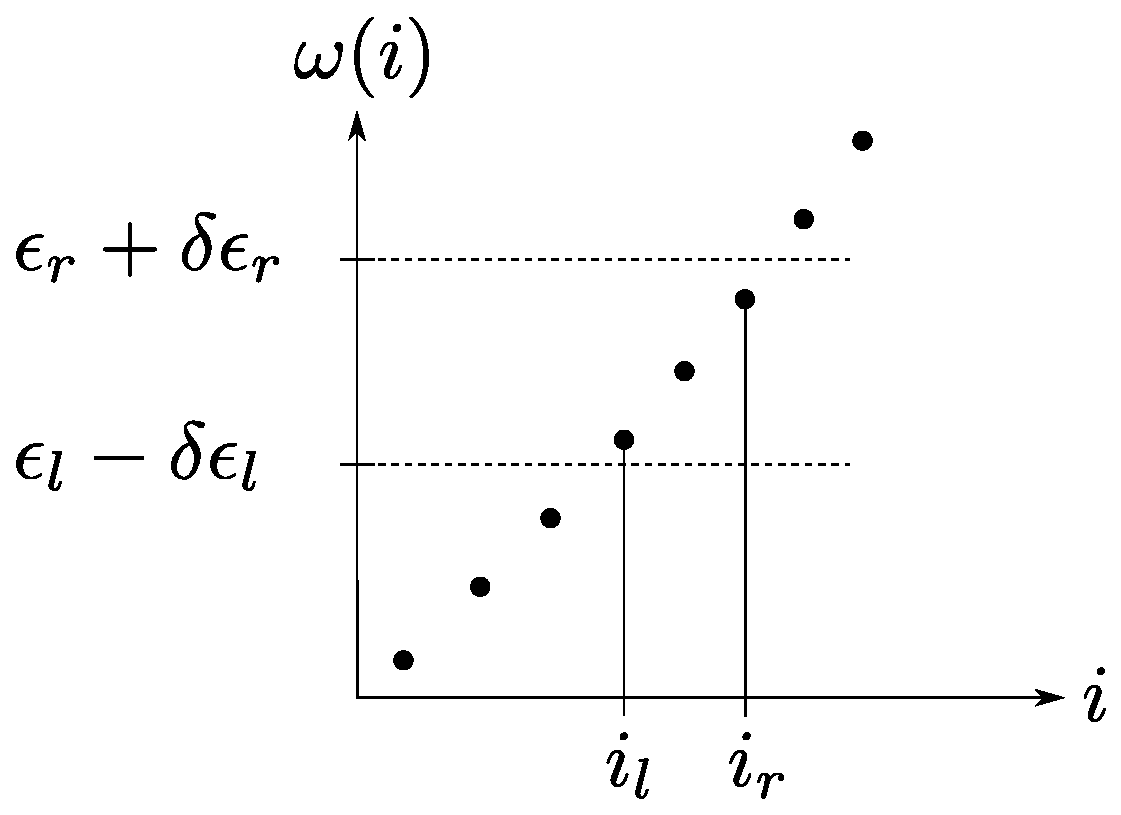
\includegraphics[width=0.4\textwidth]{pics/subgrid_inserting.eps}
	\caption{Inserting of a subgrid}
	\label{fig:subgrid_inserting}
\end{figure}
The indices $i_l$ and $i_r$ are obtained by
\begin{align*}
	\omega(i_l) & > \epsilon_l - \delta \epsilon_l \quad \text{with } i_l \text{ minimal} \\
	\omega(i_r) & < \epsilon_r + \delta \epsilon_r \quad \text{with } i_r \text{ maximal} \\
\end{align*}
where the machine precision buffer $\delta$ ensures that the resulting grid point difference ($\sim$~weights) does not become too small. 
The difference in the overall grid point number is then given by
\[
	N_R=N +1 - (i_r-i_l+1)
\]
The subgrid is inserted into the base grid at the index $i_l$. The resulting grid $\tilde \omega(i)$ is then given by
\[
	\tilde \omega(i)=\begin{cases}
			\omega(i) \quad & i = 0,\dots,i_l-1 \\
			\epsilon(i-i_l) \quad & i=i_l,\dots,i_l+N\\
			\omega(i-N_R) \quad & i=i_l+N+1,\dots,M+N_R
 	          \end{cases}
\]
The grid $\tilde \omega(i)$ then serves as a basic grid for the insertion of the next subgrid. Nevertheless if there is more than one subgrid, there is an additional subtlety which has to be taken into account: If one inserts a subgrid left from a subgrid which was inserted earlier, one has to shift the indices $i_l$ and $i_r$ for the latter one by the number of replaced grid points $N_R$ of the former one. This means, that if one adds a subgrid with $N_R^\text{new}$, one has to shift the indices $i_l$ and $i_r$ of all subgrids which lie right of the former one by
\begin{align*}
	i_l &\to i_l + N_R^\text{new} \\
	i_r &\to i_r + N_R^\text{new} \\
\end{align*}
By this procedure the multigrid is build up out of several subgrids and the basic grid.

\section{Inverse of the multigrid}\label{sec:inverse_of_the_multigrid}
\index{Inverse of the multigrid}
In this section we will show how to calculate the inverse $i(\omega)$ of a multigrid which consists of a basic grid and several subgrids. As an example we take the multigrid from listing \ref{lst:replace_gr}, see figure \ref{fig:inverse}.

\begin{figure}[h]
	\centering
	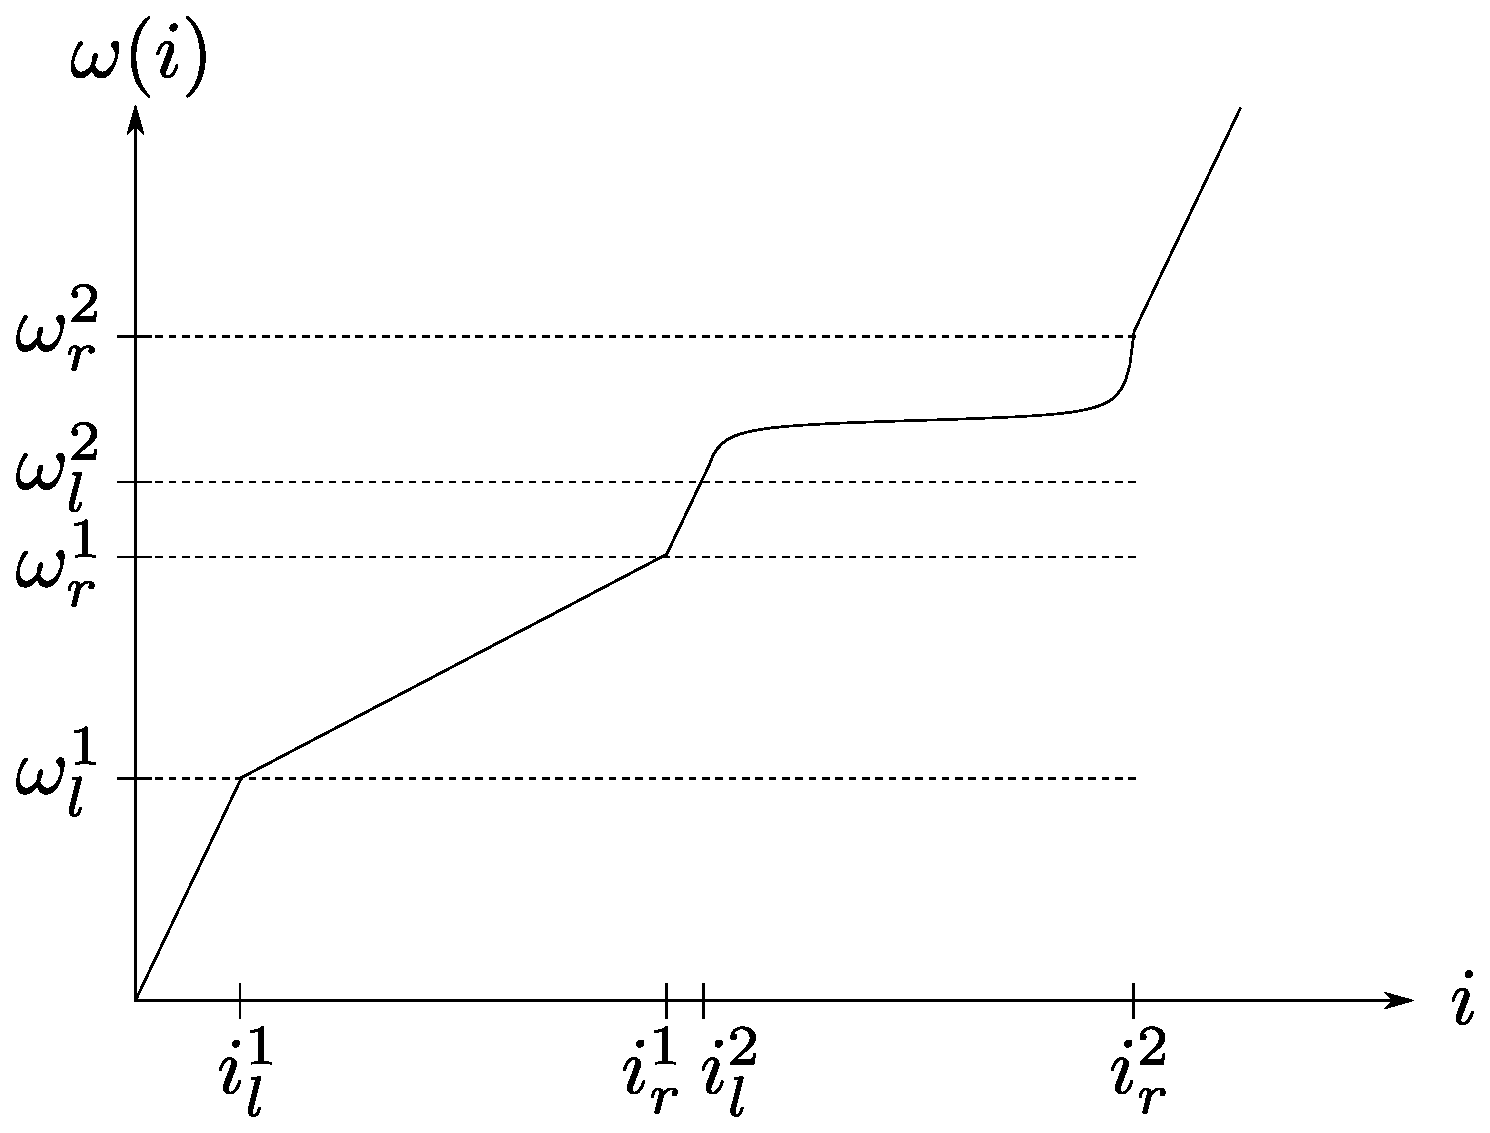
\includegraphics[width=0.5\textwidth]{pics/inverse.eps}
	\caption{Calculating the inverse mapping of a multigrid}
	\label{fig:inverse}
\end{figure}

There is a equidistant basic grid and two subgrids, an equidistant and a tangential one. We will denote the basic grid by $\omega^0(i)$, the equidistant subgrid by $\omega^1(i)$ and the tangential subgrid by $\omega^2(i)$. The corresponding inverse mappings are denoted by $i^0(\omega)$ for the basic grid, $i^1(\omega)$ for the equidistant subgrid and $i^2(\omega)$ for the tangential subgrid. In order to calculate the inverse of a given value $\omega$ one has to find out, if $\omega$ lies in one of the subgrid regions. And if this is the case, in which subgrid. Otherwise, one uses the inverse of the basic grid $i^0(\omega)$. The resulting inverse mapping is then given by
\begin{equation}\label{eqn:inverse}
	i(\omega)=\begin{cases}
			i^1(\omega) + i_l^1 \quad & \omega \in [\omega_l^1, \omega_r^1]\\
			i^2(\omega) + i_l^2 \quad & \omega \in [\omega_l^2, \omega_r^2]\\
			i^0(\omega) + N_S \quad & \omega \notin [\omega_l^1, \omega_r^1] \cup [\omega_l^2, \omega_r^2]
	          \end{cases}
\end{equation}
Where $N_S$ is the sum of all numbers of replaced points $N_R^k$ which correspond to subgrids $k$, which are left of $\omega$, i.e. which fulfill $\omega_r^k<\omega$:
\[
	N_S=\sum_{\substack{k\\ \omega_r^k<\omega}} N_R^k
\]
The generalization to an arbitrary number of subgrids it straight forward. Now it is clear, why the subgrids contain $i_l$ and $N_R$: They are directly used in the calculation of the inverse mapping.

\section{Fundamental and special grid regions}\label{sec:fundamental_and_special_grid_regions_2}
\index{Fundamental grid regions}
\index{Special grid regions}
The above multigrid was comprised of a basic grid and several subgrids. Up to now these subgrids were build out of fundamental grid regions. Therefore they are so called fundamental subgrids and we will call the resulting grid a fundamental grid. In the last section we have shown how to calculate the inverse of such a fundamental grid. Nothing prevents us from taking this fundamental grid as a basic grid for inserting more subgrids. In accordance to the special grid regions introduced in the last chapter, we will call them special subgrids. After the selection and cutting procedure the special grid regions are mapped onto special subgrids. In the same way the fundamental subgrids were inserted into the basic grid to form the fundamental grid, the special subgrids are inserted into the fundamental grid to form the resulting multigrid. While calling the inverse of a value $\omega$ of a multigrid, the algorithm  will begin by checking weather $\omega$ is inside one of the special subgrids (just like for the fundamental subgrids in equation \ref{eqn:inverse}). If this is the case it will calculate the inverse mapping of the subgrids directly (again, just like in equation \ref{eqn:inverse}). Otherwise it will call the inverse mapping of the fundamental grid (just like the inverse of the basic grid $i^0(\omega)$ is called in \ref{eqn:inverse}). The calculation of the inverse of the fundamental grid is was explained in the last sections.



